Generalization is a core concept when talking about the \textit{k-anonymity with generalization} problem.
The algorithm described in Chapter~\ref{ch:chapter_algorithm} uses generalization at its core: both to determine which rows to put into the same partition, and during the final step when the original rows are anonymized.

\subsection{Generalization API requirements}\label{subsec:generalization_requirements}
The library needs to provide a way for the API user to define how to generalize certain data types in their schema.
The implementation also needs to be flexible, but convenient and easy-to-use at the same time.
We want to make sure, that the implementation can satisfy at least the following requirements:

\begin{itemize}
    \setstretch{1.0}
    \item supports \textbf{generalization hierarchy}, with convenient declaration
    \item supports \textbf{suppression}
    \item supports \textbf{sets, ranges}
    \item supports \textbf{text}
    \item supports \textbf{non}-hierarchy based generalization
    \item custom generalizers can be created by \textbf{implementing an interface}
\end{itemize}

Until now we have only discussed \textit{hierarchy}-based generalization, and for the theoretical discussion of the anonymization algorithm it was perfectly sufficient.
You can create a generalization hierarchy for basically any data type --- even though the number of levels and the number of partitions on a given level may end up very large, or even infinite.

It is important to note however, that in real-life scenarios this is not always feasible.
Storage, operating memory and computing time is finite, which means that for some dimensions (like \textit{text}) we will need to apply a different type of abstraction.

\subsection{Generalization implementation}\label{subsec:generalization-implementation}
Based on the requirements outlined in~\ref{subsec:generalization_requirements} we can define the interface of a \texttt{Generalizer}.
Note, that since Go is not a classic object oriented language, a traditional class-hierarchy is not present in the design.
What we do have in our toolkit are \textit{interfaces} and \textit{composition}.

We define the \texttt{Generalizer} interface with the following operations (refer to Figure~\ref{fig:generalization_package}):
\begin{enumerate}
    \setstretch{1.0}
    \item generalize a partition \textit{n} times
    \item get the maximum number of levels of generalization
\end{enumerate}
Remember, that a partition can either contain a single value, or a set of values, so it makes sense that the \texttt{Generalize} method takes and returns a \texttt{Partition}.
It is also essential to know the maximum levels of generalization in advance, otherwise we wouldn't be able to compute the scaled generalization cost when comparing two partitions.
There is a third convenience method on the interface which defines how to create a \texttt{Partition} from a raw value.
The actual implementation of this may vary in each type that implements the interface.

\vspace{\baselineskip}
\begin{figure}
    \centering
    \includegraphics[width=\textwidth]{lib-generalizer.png}
    \caption{The generalization package}\label{fig:generalization_package}
\end{figure}



\subsection{Suppressor}
\begin{lstlisting}[caption=Suppresor implementation,label=lst:suppressor,float,floatplacement=H]
type Suppressor struct {
}

func (s *Suppressor) Generalize(p partition.Partition, n int) partition.Partition {
    if n == 0 {
        return p
    }
    if n == 1 {
        return s.InitItem("*")
    }
    return nil
}

func (s *Suppressor) Levels() int {
    return 2
}

func (s *Suppressor) InitItem(item interface{}) partition.Partition {
    return partition.NewItem(item)
}
\end{lstlisting}

\subsection{HierarchyGeneralizer}\label{subsec:hierarchy_generalizer}
\texttt{HierarchyGeneralizer} represents generalization hierarchies in the classic sense that has been outlined in~\ref{subsec:data_model}.
This generalizer will \textit{contain} an actual \texttt{Hierarchy} --- as seen on Figure~\ref{fig:generalization_package}.
The \texttt{Hierarchy} interface has functions to navigate the partitions within the hierarchy based on the parent-child relationships, a function to return the number of levels within the hierarchy and additional helper functions.
The \texttt{hierarchy} package also contains helper functions to make it easy for the end-user to build it from a set of items.

\paragraph{Manual hierarchy:} We will now show how to manually declare a simple grade hierarchy similar to the one introduced on Figure~\ref{fig:grades-hierarchy}, albeit with a lesser number of grades for simplicity's sake. The full code listing can be seen on Listing~\ref{lst:grade_hierarchy}.

\begin{lstlisting}[caption=Grade Hierarchy,label=lst:grade_hierarchy]
func GetGradeHierarchy() Hierarchy {
    h, _ := Build(
        partition.NewSet("A+", "A", "A-", "B+", "B", "B-", "C+", "C", "C-"),
            N(partition.NewSet("A+", "A", "A-"),
                N(partition.NewSet("A+")),
                N(partition.NewSet("A")),
                N(partition.NewSet("A-"))),
        N(partition.NewSet("B+", "B", "B-"),
            N(partition.NewSet("B+")),
            N(partition.NewSet("B")),
            N(partition.NewSet("B-"))),
        N(partition.NewSet("C+", "C", "C-"),
            N(partition.NewSet("C+")),
            N(partition.NewSet("C")),
            N(partition.NewSet("C-"))))
    return h
}
\end{lstlisting}

In order to build the hierarchy, we need to describe it from top to bottom.
Recall, that the top level of the hierarchy contains a single partition with every item in the domain.
We then add the children of this partition as new sets, continuing until we reach the lowest level, where each partition contains only a single item.

\paragraph{Automatic hierarchy:} another, more convenient way to build a hierarchy is by using the included \texttt{AutoBuild} function. It takes two parameters: the amount of children a node should have, and a variadic array of the items to partition. The function will build a valid hierarchy on-the-fly by splitting the set of items to the specified child partitions on each level, until only singleton partitions remain. (Note, that we may still get an error in case there is a problem with the arguments, for example when the desired child count is larger than the available items.) The builder may create partitions with less than the specified amount of children in cases when there aren't enough items. This often happens when the original number of items is not divisible by the desired child count.

 We now show how to build the same grade hierarchy automatically. Listing~\ref{lst:auto_build} demonstrates how to specify the child count and the items. By passing in \textit{3} as the desired child count we achieve the exact same result as the previous example.

\begin{lstlisting}[caption=Hierarchy with the AutoBuild function,label=lst:auto_build]
h, err := hierarchy.AutoBuild(3, "A+", "A", "A-", "B+", "B", "B-", "C+", "C", "C-")
\end{lstlisting}

\paragraph{Validation} A hierarchy will also be \textit{validated} when it is built.
Validation will enforce, that:
\begin{itemize}
    \setstretch{1.0}
    \item an item can only appear once on a given level
    \item the superset of partitions on each level contains all items from the domain
\end{itemize}

\subsection{RangeGeneralizer}
\begin{figure}[H]
    \centering


    \tikzset{every picture/.style={line width=0.75pt}} %set default line width to 0.75pt

    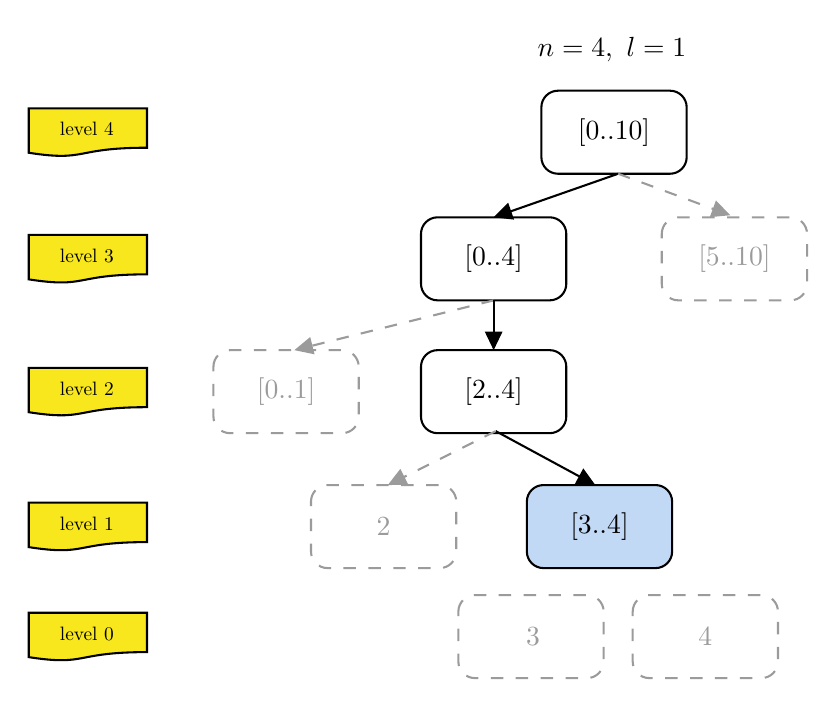
\begin{tikzpicture}[x=0.75pt,y=0.75pt,yscale=-1,xscale=1]
        %uncomment if require: \path (0,340); %set diagram left start at 0, and has height of 340

        %Rounded Rect [id:dp41297758491075554]
        \draw  [color={rgb, 255:red, 0; green, 0; blue, 0 }  ,draw opacity=1 ] (284,48) .. controls (284,43.58) and (287.58,40) .. (292,40) -- (346,40) .. controls (350.42,40) and (354,43.58) .. (354,48) -- (354,72) .. controls (354,76.42) and (350.42,80) .. (346,80) -- (292,80) .. controls (287.58,80) and (284,76.42) .. (284,72) -- cycle ;
        %Rounded Rect [id:dp6520424082590635]
        \draw   (226,109) .. controls (226,104.58) and (229.58,101) .. (234,101) -- (288,101) .. controls (292.42,101) and (296,104.58) .. (296,109) -- (296,133) .. controls (296,137.42) and (292.42,141) .. (288,141) -- (234,141) .. controls (229.58,141) and (226,137.42) .. (226,133) -- cycle ;
        %Rounded Rect [id:dp17376535076708577]
        \draw  [color={rgb, 255:red, 155; green, 155; blue, 155 }  ,draw opacity=1 ][dash pattern={on 4.5pt off 4.5pt}] (342,109) .. controls (342,104.58) and (345.58,101) .. (350,101) -- (404,101) .. controls (408.42,101) and (412,104.58) .. (412,109) -- (412,133) .. controls (412,137.42) and (408.42,141) .. (404,141) -- (350,141) .. controls (345.58,141) and (342,137.42) .. (342,133) -- cycle ;
        %Rounded Rect [id:dp6626394915573943]
        \draw   (226,173) .. controls (226,168.58) and (229.58,165) .. (234,165) -- (288,165) .. controls (292.42,165) and (296,168.58) .. (296,173) -- (296,197) .. controls (296,201.42) and (292.42,205) .. (288,205) -- (234,205) .. controls (229.58,205) and (226,201.42) .. (226,197) -- cycle ;
        %Rounded Rect [id:dp6613554759465123]
        \draw  [color={rgb, 255:red, 155; green, 155; blue, 155 }  ,draw opacity=1 ][dash pattern={on 4.5pt off 4.5pt}] (126,173) .. controls (126,168.58) and (129.58,165) .. (134,165) -- (188,165) .. controls (192.42,165) and (196,168.58) .. (196,173) -- (196,197) .. controls (196,201.42) and (192.42,205) .. (188,205) -- (134,205) .. controls (129.58,205) and (126,201.42) .. (126,197) -- cycle ;
        %Rounded Rect [id:dp18103482508891444]
        \draw  [color={rgb, 255:red, 155; green, 155; blue, 155 }  ,draw opacity=1 ][dash pattern={on 4.5pt off 4.5pt}] (173,238) .. controls (173,233.58) and (176.58,230) .. (181,230) -- (235,230) .. controls (239.42,230) and (243,233.58) .. (243,238) -- (243,262) .. controls (243,266.42) and (239.42,270) .. (235,270) -- (181,270) .. controls (176.58,270) and (173,266.42) .. (173,262) -- cycle ;
        %Rounded Rect [id:dp6156099131399975]
        \draw  [color={rgb, 255:red, 0; green, 0; blue, 0 }  ,draw opacity=1 ][fill={rgb, 255:red, 193; green, 217; blue, 245 }  ,fill opacity=1 ] (277,238) .. controls (277,233.58) and (280.58,230) .. (285,230) -- (339,230) .. controls (343.42,230) and (347,233.58) .. (347,238) -- (347,262) .. controls (347,266.42) and (343.42,270) .. (339,270) -- (285,270) .. controls (280.58,270) and (277,266.42) .. (277,262) -- cycle ;
        %Straight Lines [id:da940569460881393]
        \draw    (321,80) -- (262.89,100.34) ;
        \draw [shift={(261,101)}, rotate = 340.71000000000004] [fill={rgb, 255:red, 0; green, 0; blue, 0 }  ][line width=0.75]  [draw opacity=0] (8.93,-4.29) -- (0,0) -- (8.93,4.29) -- cycle    ;

        %Straight Lines [id:da19886917638438795]
        \draw [color={rgb, 255:red, 155; green, 155; blue, 155 }  ,draw opacity=1 ] [dash pattern={on 4.5pt off 4.5pt}]  (321,80) -- (373.12,99.31) ;
        \draw [shift={(375,100)}, rotate = 200.32] [fill={rgb, 255:red, 155; green, 155; blue, 155 }  ,fill opacity=1 ][line width=0.75]  [draw opacity=0] (8.93,-4.29) -- (0,0) -- (8.93,4.29) -- cycle    ;

        %Straight Lines [id:da7809582170361684]
        \draw [color={rgb, 255:red, 155; green, 155; blue, 155 }  ,draw opacity=1 ] [dash pattern={on 4.5pt off 4.5pt}]  (261,141) -- (166.94,164.51) ;
        \draw [shift={(165,165)}, rotate = 345.96000000000004] [fill={rgb, 255:red, 155; green, 155; blue, 155 }  ,fill opacity=1 ][line width=0.75]  [draw opacity=0] (8.93,-4.29) -- (0,0) -- (8.93,4.29) -- cycle    ;

        %Straight Lines [id:da49593042124322273]
        \draw    (261,141) -- (261,163) ;
        \draw [shift={(261,165)}, rotate = 270] [fill={rgb, 255:red, 0; green, 0; blue, 0 }  ][line width=0.75]  [draw opacity=0] (8.93,-4.29) -- (0,0) -- (8.93,4.29) -- cycle    ;

        %Straight Lines [id:da07216174009388476]
        \draw    (262,204) -- (308.24,229.05) ;
        \draw [shift={(310,230)}, rotate = 208.44] [fill={rgb, 255:red, 0; green, 0; blue, 0 }  ][line width=0.75]  [draw opacity=0] (8.93,-4.29) -- (0,0) -- (8.93,4.29) -- cycle    ;

        %Straight Lines [id:da9300341613494139]
        \draw [color={rgb, 255:red, 155; green, 155; blue, 155 }  ,draw opacity=1 ] [dash pattern={on 4.5pt off 4.5pt}]  (262,204) -- (211.79,229.11) ;
        \draw [shift={(210,230)}, rotate = 333.43] [fill={rgb, 255:red, 155; green, 155; blue, 155 }  ,fill opacity=1 ][line width=0.75]  [draw opacity=0] (8.93,-4.29) -- (0,0) -- (8.93,4.29) -- cycle    ;

        %Flowchart: Document [id:dp6500761765411522]
        \draw  [fill={rgb, 255:red, 248; green, 231; blue, 28 }  ,fill opacity=1 ] (37,48.5) -- (94,48.5) -- (94,67.47) .. controls (58.38,67.47) and (65.5,74.32) .. (37,69.89) -- cycle ;

        %Flowchart: Document [id:dp5580407874202131]
        \draw  [fill={rgb, 255:red, 248; green, 231; blue, 28 }  ,fill opacity=1 ] (37,109.5) -- (94,109.5) -- (94,128.48) .. controls (58.38,128.48) and (65.5,135.32) .. (37,130.89) -- cycle ;

        %Flowchart: Document [id:dp3741114720480607]
        \draw  [fill={rgb, 255:red, 248; green, 231; blue, 28 }  ,fill opacity=1 ] (37,173.5) -- (94,173.5) -- (94,192.48) .. controls (58.38,192.48) and (65.5,199.32) .. (37,194.89) -- cycle ;

        %Flowchart: Document [id:dp020109097297930534]
        \draw  [fill={rgb, 255:red, 248; green, 231; blue, 28 }  ,fill opacity=1 ] (37,238.5) -- (94,238.5) -- (94,257.48) .. controls (58.38,257.48) and (65.5,264.32) .. (37,259.89) -- cycle ;

        %Flowchart: Document [id:dp06728244444869125]
        \draw  [fill={rgb, 255:red, 248; green, 231; blue, 28 }  ,fill opacity=1 ] (37,291.5) -- (94,291.5) -- (94,310.48) .. controls (58.38,310.48) and (65.5,317.32) .. (37,312.89) -- cycle ;

        %Rounded Rect [id:dp005401328342101053]
        \draw  [color={rgb, 255:red, 155; green, 155; blue, 155 }  ,draw opacity=1 ][dash pattern={on 4.5pt off 4.5pt}] (244,291) .. controls (244,286.58) and (247.58,283) .. (252,283) -- (306,283) .. controls (310.42,283) and (314,286.58) .. (314,291) -- (314,315) .. controls (314,319.42) and (310.42,323) .. (306,323) -- (252,323) .. controls (247.58,323) and (244,319.42) .. (244,315) -- cycle ;
        %Rounded Rect [id:dp20978566864575288]
        \draw  [color={rgb, 255:red, 155; green, 155; blue, 155 }  ,draw opacity=1 ][dash pattern={on 4.5pt off 4.5pt}] (328,291) .. controls (328,286.58) and (331.58,283) .. (336,283) -- (390,283) .. controls (394.42,283) and (398,286.58) .. (398,291) -- (398,315) .. controls (398,319.42) and (394.42,323) .. (390,323) -- (336,323) .. controls (331.58,323) and (328,319.42) .. (328,315) -- cycle ;

        % Text Node
        \draw (318,20) node  [align=left] {$\displaystyle n=4,\ l=1$};
        % Text Node
        \draw (377,121) node [color={rgb, 255:red, 155; green, 155; blue, 155 }  ,opacity=1 ] [align=left] {[5..10]};
        % Text Node
        \draw (261,121) node  [align=left] {[0..4]};
        % Text Node
        \draw (319,60) node [color={rgb, 255:red, 0; green, 0; blue, 0 }  ,opacity=1 ] [align=left] {[0..10]};
        % Text Node
        \draw (261,185) node  [align=left] {[2..4]};
        % Text Node
        \draw (161,185) node [color={rgb, 255:red, 155; green, 155; blue, 155 }  ,opacity=1 ] [align=left] {[0..1]};
        % Text Node
        \draw (208,250) node [color={rgb, 255:red, 155; green, 155; blue, 155 }  ,opacity=1 ] [align=left] {2};
        % Text Node
        \draw (312,250) node  [align=left] {[3..4]};
        % Text Node
        \draw (65,58.5) node [scale=0.7] [align=left] {level 4};
        % Text Node
        \draw (65,119.5) node [scale=0.7] [align=left] {level 3};
        % Text Node
        \draw (65,183.5) node [scale=0.7] [align=left] {level 2};
        % Text Node
        \draw (65,248.5) node [scale=0.7] [align=left] {level 1};
        % Text Node
        \draw (65,301.5) node [scale=0.7] [align=left] {level 0};
        % Text Node
        \draw (280,303) node [color={rgb, 255:red, 155; green, 155; blue, 155 }  ,opacity=1 ] [align=left] {3};
        % Text Node
        \draw (363,303) node [color={rgb, 255:red, 155; green, 155; blue, 155 }  ,opacity=1 ] [align=left] {4};


    \end{tikzpicture}
    \caption{Range generalizer example}\label{fig:range_generalizer}
\end{figure}

\subsection{PrefixGeneralizer}\label{subsec:prefix_generalizer}
The \texttt{PrefixGeneralizer} is another built-in generalizer, that does not rely on a fixed hierarchy. It deals with generalizing plain text data. As the name suggests, it will try to use different sized prefixes to see if two different strings can be collapsed into the same partition.

The input text will be interpreted as a series of words. The generalizer has a \texttt{MaxWords} setting, and it cannot handle text that has a larger word count. Note, that the actual length of words in characters is \textit{irrelevant} for this generalizer, and is only bounded by operative memory.

\paragraph{Example:} the example on Figure~\ref{fig:prefix_generalizer_1} shows how the prefix generalizer transforms two different sentences when different levels of generalization \textit{l} are selected. We assume, that \(MaxWords = 5\) for this example.

The first sentence only contains 3 words, so the \texttt{PrefixGeneralizer} will pad the last two slots. This makes it easy to compare the two sentences word-by-word. On levels 0, 1 and 2 the string prefixes are not equal. On level 3 the two strings are equal. Calculating the generalization cost for the two values would also be pretty simple: we divide the lowest level of generalization which assigns the two items into the same partition by the maximum levels of generalization: \(h/l_{\max} = 3/5\).

\vspace{\baselineskip}
\input{chapter03/figures/prefix-generalizer-1.tex}

Figure~\ref{fig:prefix_generalizer_2} illustrates what happens when the two strings differ in all prefixes. In this case the cost of generalization will be \(h/l_{\max} = 1 \), and both of the two strings are \textit{suppressed} (replaced with the ``*'' token).

\vspace{\baselineskip}
\begin{figure}[ht]
    \centering


\tikzset{every picture/.style={line width=0.75pt}} %set default line width to 0.75pt

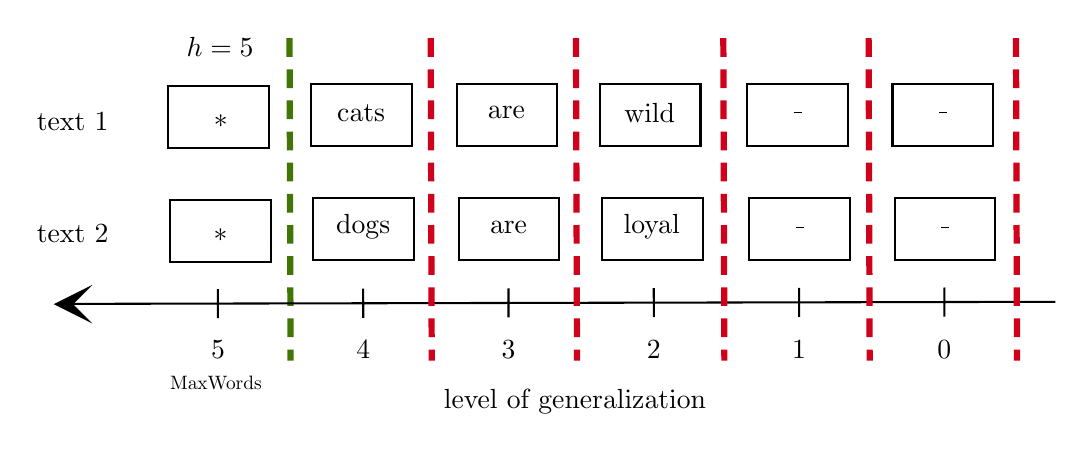
\begin{tikzpicture}[x=0.75pt,y=0.75pt,yscale=-1,xscale=1]
%uncomment if require: \path (0,316); %set diagram left start at 0, and has height of 316

%Shape: Rectangle [id:dp5153514125810188]
\draw   (210,42) -- (258.5,42) -- (258.5,72) -- (210,72) -- cycle ;

%Shape: Rectangle [id:dp3792357730299869]
\draw   (280,42) -- (328.5,42) -- (328.5,72) -- (280,72) -- cycle ;

%Shape: Rectangle [id:dp5360715303240602]
\draw   (349,42) -- (397.5,42) -- (397.5,72) -- (349,72) -- cycle ;

%Shape: Rectangle [id:dp39881760222299123]
\draw   (420,42) -- (468.5,42) -- (468.5,72) -- (420,72) -- cycle ;

%Shape: Rectangle [id:dp24969521881010048]
\draw   (490,42) -- (538.5,42) -- (538.5,72) -- (490,72) -- cycle ;

%Shape: Rectangle [id:dp1737030576273597]
\draw   (211,97) -- (259.5,97) -- (259.5,127) -- (211,127) -- cycle ;

%Shape: Rectangle [id:dp2321963000324494]
\draw   (281,97) -- (329.5,97) -- (329.5,127) -- (281,127) -- cycle ;

%Shape: Rectangle [id:dp6988583402431512]
\draw   (350,97) -- (398.5,97) -- (398.5,127) -- (350,127) -- cycle ;

%Shape: Rectangle [id:dp7718120947102272]
\draw  [fill={rgb, 255:red, 255; green, 255; blue, 255 }  ,fill opacity=1 ] (421,97) -- (469.5,97) -- (469.5,127) -- (421,127) -- cycle ;

%Shape: Rectangle [id:dp4373041939092148]
\draw  [fill={rgb, 255:red, 255; green, 255; blue, 255 }  ,fill opacity=1 ] (491,97) -- (539.5,97) -- (539.5,127) -- (491,127) -- cycle ;

%Shape: Rectangle [id:dp7370656893447207]
\draw   (141,43) -- (189.5,43) -- (189.5,73) -- (141,73) -- cycle ;
%Shape: Rectangle [id:dp45288136830178805]
\draw   (142,98) -- (190.5,98) -- (190.5,128) -- (142,128) -- cycle ;
%Straight Lines [id:da8313945580724125]
\draw [color={rgb, 255:red, 65; green, 117; blue, 5 }  ,draw opacity=1 ][line width=2.25]  [dash pattern={on 6.75pt off 4.5pt}]  (199.5,20) -- (200,175.33) ;


%Straight Lines [id:da846675768790583]
\draw    (95,148) -- (568.5,147) (164.99,140.85) -- (165.01,154.85)(234.98,140.7) -- (235.01,154.7)(304.98,140.56) -- (305.01,154.56)(374.98,140.41) -- (375.01,154.41)(444.98,140.26) -- (445.01,154.26)(514.98,140.11) -- (515.01,154.11) ;


\draw  [fill={rgb, 255:red, 0; green, 0; blue, 0 }  ,fill opacity=1 ] (102,155.67) -- (87,148.17) -- (102,140.67) -- (94.5,148.17) -- cycle ;
%Straight Lines [id:da7170976620765326]
\draw [color={rgb, 255:red, 208; green, 2; blue, 27 }  ,draw opacity=1 ][line width=2.25]  [dash pattern={on 6.75pt off 4.5pt}]  (408.5,20) -- (409,175.33) ;


%Straight Lines [id:da920755443743104]
\draw [color={rgb, 255:red, 208; green, 2; blue, 27 }  ,draw opacity=1 ][line width=2.25]  [dash pattern={on 6.75pt off 4.5pt}]  (478.5,20) -- (479,175.33) ;


%Straight Lines [id:da6869452406118943]
\draw [color={rgb, 255:red, 208; green, 2; blue, 27 }  ,draw opacity=1 ][line width=2.25]  [dash pattern={on 6.75pt off 4.5pt}]  (549.5,20) -- (550,175.33) ;


%Straight Lines [id:da15957952333358016]
\draw [color={rgb, 255:red, 208; green, 2; blue, 27 }  ,draw opacity=1 ][line width=2.25]  [dash pattern={on 6.75pt off 4.5pt}]  (337.5,20) -- (338,175.33) ;


%Straight Lines [id:da5495481423548718]
\draw [color={rgb, 255:red, 208; green, 2; blue, 27 }  ,draw opacity=1 ][line width=2.25]  [dash pattern={on 6.75pt off 4.5pt}]  (267.5,20) -- (268,175.33) ;



% Text Node
\draw (304,56) node  [align=left] {are};
% Text Node
\draw (234,56) node  [align=left] {cats};
% Text Node
\draw (373,56) node  [align=left] {wild};
% Text Node
\draw (444,56) node  [align=left] {\_};
% Text Node
\draw (514,56) node  [align=left] {\_};
% Text Node
\draw (515,111) node  [align=left] {\_};
% Text Node
\draw (445,111) node  [align=left] {\_};
% Text Node
\draw (374,111) node  [align=left] {loyal};
% Text Node
\draw (305,111) node  [align=left] {are};
% Text Node
\draw (235,111) node  [align=left] {dogs};
% Text Node
\draw (337,195) node  [align=left] {level of generalization};
% Text Node
\draw (235,170) node  [align=left] {4};
% Text Node
\draw (305,170) node  [align=left] {3};
% Text Node
\draw (375,170) node  [align=left] {2};
% Text Node
\draw (445,170) node  [align=left] {1};
% Text Node
\draw (515,170) node  [align=left] {0};
% Text Node
\draw (165,170) node  [align=left] {5};
% Text Node
\draw (166.25,117) node  [align=left] {*};
% Text Node
\draw (166.33,62) node  [align=left] {*};
% Text Node
\draw (95,60) node  [align=left] {text 1};
% Text Node
\draw (95,114) node  [align=left] {text 2};
% Text Node
\draw (164,186) node [scale=0.7] [align=left] {MaxWords};
% Text Node
\draw (166,24) node  [align=left] {$\displaystyle h=5$};


\end{tikzpicture}

    \caption{Prefix generalizer (h=5)}\label{fig:prefix_generalizer_2}
\end{figure}

\subsection{Custom Generalizers}
Finally, if none of the built-in generalization techniques are adequate for a certain use case, the user of the library can still implement the \texttt{Generalizer} interface to provide a custom logic.

Recall from Section~\ref{sec:generalization}, that in order to properly implement the \texttt{Generalizer} interface, one has to implement the following methods:

\underline{\texttt{Levels () int}}: \\
This method should return the maximum number of times the generalizer can generalize the values. In hierarchy based generalizers it is usually the number of levels in the tree. It is important to note, that the levels are zero-indexed, which needs to be taken account when calculating the number of levels with a non-hierarchy based logic.

\underline{\texttt{Generalize (Partition, int) Partition}}: \\
This method should generalize the input partition n times (providing that \(n \le Levels ()\)) and return the resulting partition. The result will be used by the core anonymization algorithm when calculating the cost graph.

\underline{\texttt{InitItem (interface\{ \}) Partition}}: \\
Implement this method to tell how to initialize a raw value. In most cases you just want to wrap it into an \texttt{Item} or \texttt{Set}.